%\section*{Administración del proyecto}
%\subsection*{Presupuesto estimado e infraestructura}
%tablas 5, 6 y 7 
%-----------------------------tabla 5-----------------------------
\begin{center}
\footnotesize
    \begin{longtable}[!htb]{| m{15em} | m{6em} | m{6em}| m{6em}|}
    \hline
    \textbf{Personal}& \textbf{\'Area de aporte} & \textbf{Instituci\'on} & \textbf{Tiempo m\'inimo}\\
    \hline\hline
    Estudiante: Barbosa Mercado José Aarón & STEM & UPIITA-IPN & 600 hrs\\
    \hline
    Estudiante: Camarena Rodríguez Alberto & STEM & UPIITA-IPN & 600 hrs\\
    \hline
    Estudiante: Muñoz Ceballos Teddy Xavier & STEM & UPIITA-IPN & 600 hrs\\
    \hline
    Estudiante: Sánchez Trujillo Daniel & STEM & UPIITA-IPN & 600 hrs\\
    \hline
    Asesor: Dr. Rafael Trovamala Landa & STEM & UPIITA-IPN/Ik'Atl & 60 hrs\\
    \hline
    Asesor: Dr. Alberto Luviano Juárez & STEM & UPIITA-IPN & 60 hrs\\
    \hline
    Especialista Externo: Rogelio Israel Quintero Tiscareño & Ingeniero en audio & Espiral Est\'ereo & 50 hrs\\
    \hline

    \caption{Tabla de recursos humanos.}
    \label{tab:RH}
    \end{longtable}
\end{center}
%-----------------------------tabla 5-----------------------------

%-----------------------------tabla 6-----------------------------
\begin{center}
\footnotesize
    \begin{longtable}[!htb]{| m{10em} | m{12em} | m{12em}|}
    \hline
    \textbf{Infraestructura}& \textbf{Desciripci\'on} & \textbf{Uso} \\
    \hline\hline
    Estudio de grabaci\'on & Recinto sobre el cual se desea hacer el tratamiento acústico. & Es el cuarto destinado sobre el que se trabajará el trabajo terminal.\\
    \hline
    Laboratorio de pesados & Taller donde se encuentran las máquinas e instrumentos. & En él, se manufacturarán las piezas.\\
    \hline

    \caption{Infraestructura para el desarrollo del proyecto.}
    \label{tab:Infraestructura}
    \end{longtable}
\end{center}
%-----------------------------tabla 6-----------------------------
%-----------------------------tabla 7-----------------------------
\begin{center}
\scriptsize
    \begin{longtable}[!htb]{| m{4em} | m{8em} | m{4.5em}| m{4em}| m{3em}| m{8em}| m{4em}|}
    \hline
    \textbf{M\'odulo}& \textbf{Material} & \textbf{Cantidad} & \textbf{Costo unitario} & \textbf{Costo total} & \textbf{Financiamiento} & \textbf{Fuente}\\
    \hline\hline
    \multirow{7}{*}{MMRP} 
    & Monitor de audio con amplificador & 1 & $\$$3,514 & $\$$3,514 & Privado & [20]\\
    \cline{2-7}
    & Micr\'ofono de condensador & 1 & $\$$3,599 & $\$$3,599 & Privado & [21]\\
    \cline{2-7}
    & Interfaz de audio & 1 & $\$$2,199 & $\$$2,199 & Privado & [22]\\
    \cline{2-7}
    & Cable XLR balanceado & 1 & $\$$167 & $\$$167 & Privado & [23]\\
    \cline{2-7}
    & Pedestal & 1 & $\$$188 & $\$$188 & Privado & [24]\\
    \cline{2-7}
    & Software generador de onda arbitraria & 1 & $\$$0 & $\$$0 & Privado & Estimado\\
    \cline{2-7}
    & Software para adquisici\'on de datos & 1 & $\$$0 & $\$$0 & Privado & Estimado\\
    \hline

    \multirow{5}{*}{MMP} 
    & Tarjeta de desarrollo & 1 & $\$$752 & $\$$752 & Propio & [25]\\
    \cline{2-7}
    & Motor & 4 & $\$$256 & $\$$1,024 & Propio & [26]\\
    \cline{2-7}
    & Panel ac\'ustico profesional de absorci\'on & 5 & $\$$673 & $\$$3,375 & Privado & [27]\\
    \cline{2-7}
    & Cople de uni\'on  & 4 & $\$$200 & $\$$800 & Propio & Estimado\\
    \cline{2-7}
    & Material de construci\'on de paneles de difusi\'on  y reflexi\'on (Madera) & 5 & $\$$385 & $\$$1,935 & Propio & [28]\\
    \hline

    & Esponja aislante & 5 & $\$$623 & $\$$3,115 & Propio & [29]\\
    \hline
    
    & Espuma absorbente & 5 & $\$$1,892 & $\$$9,460 & Propio & [30]\\
    \hline

    MCI & Software de control  & 1 & $\$$0 & $\$$0 & Privado & Estimado\\
    \hline
    MPC & Software de interfaz & 1 & $\$$0 & $\$$0 & Privado & Estimado\\
    \hline
    
    \caption{Presupuesto estimado}
    \label{tab:Presupuesto}
    \end{longtable}
\end{center}


%-----------------------------tabla 7-----------------------------
El costo total aproximado del proyecto sería $\$30,108$

\subsection*{Planeaci\'on de actividades}
\begin{figure}[!htb]
    \centering
    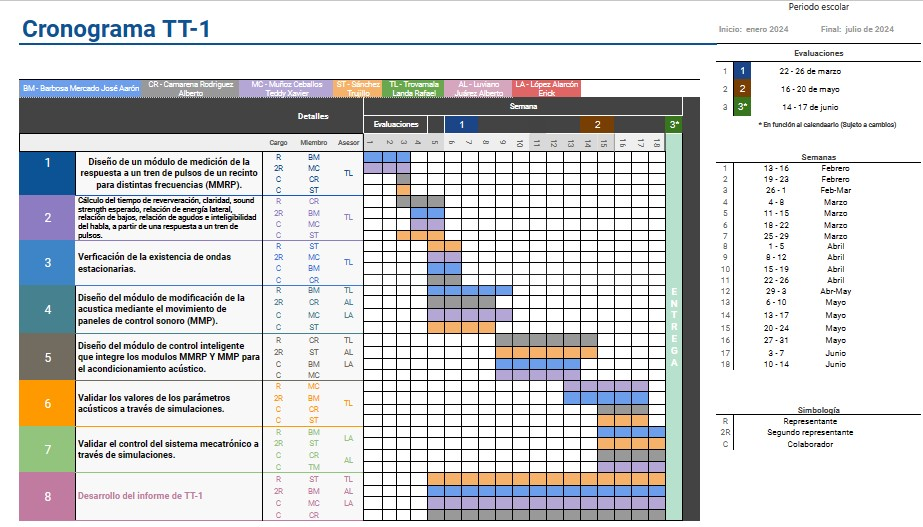
\includegraphics[width=1\textwidth]{imagenes/Protocolo21.jpg}
    \caption{\footnotesize Cronograma de actividades para TT1.}
\end{figure}
\FloatBarrier

\begin{figure}[!htb]
    \centering
    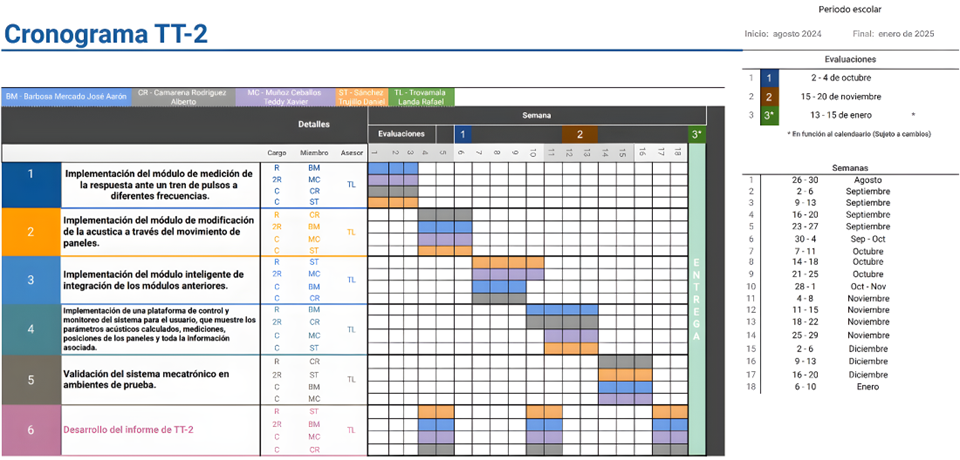
\includegraphics[width=1\textwidth]{imagenes/Protocolo22.png}
    \caption{\footnotesize Cronograma de actividades para TT2.}
\end{figure}
\FloatBarrier

\section{Diseño del sistema}
\subsection{Diseño conceptual}
\subsubsection{Necesidades y requerimientos}
\subsubsection{Arquitectura funcional}
\subsubsection{Propuestas solución}

$S_{1}$: Sistema de medición de la acústica \\
\tab    $M_{1}$: Modulo de generación del tren de pulsos \\
\tab    $M_{2}$: Modulo de medición de la respuesta \\
\tab    $M_{3}$: Modulo de procesado y calculo \\
$S_{2}$: Sistema de control y procesado \\
$S_{3}$: Sistema de movimiento de paneles acústicos \\
$S_{4}$: Sistema de interfaz humano-maquina \\
\tab    $M_{4}$: Modulo de despliegue de información
$S_{5}$: Sistema de gestión de la energía \\

Se realizo una matriz de trazabilidad para verificar que los sistemas y módulos propuestos para la arquitectura física cumplieran con las funciones a ser desempeñadas.
%----------------------------------------------------